
%(BEGIN_QUESTION)
% Copyright 2010, Tony R. Kuphaldt, released under the Creative Commons Attribution License (v 1.0)
% This means you may do almost anything with this work of mine, so long as you give me proper credit

Suppose a technician needs to test a pH transmitter, but has no pH probes to connect to its input.  Instead, she decides to build a voltage divider network to simulate the voltage levels generated by a pH probe at room temperature (25 $^{o}$C):

$$\includegraphics[width=15.5cm]{i01701x01.eps}$$

Sketch the necessary wire connections to simulate a condition of 10.5 pH at the pH transmitter's ``pH'' terminals, assuming the glass pH electrode normally generates a negative potential compared to the reference electrode while sensing an alkaline solution.  Also, calculate the necessary resistor value ($R$) to generate the required millivoltage.

\vskip 10pt

$R$ = \underbar{\hskip 50pt} $\Omega$
\underbar{file i01701}
%(END_QUESTION)





%(BEGIN_ANSWER)

This is just one possible wiring solution:

$$\includegraphics[width=15.5cm]{i01701x02.eps}$$

The resistor network must generate a signal of -207.11 millivolts, requiring a resistor with a value of {\bf 8704.66 ohms}.

\vskip 10pt

I recommend 5 points for the sketch and 5 points for the calculated resistor value.

%(END_ANSWER)





%(BEGIN_NOTES)

{\bf This question is intended for exams only and not worksheets!}.

%(END_NOTES)

